\documentclass[12pt]{article}
\usepackage[utf8]{inputenc}
\usepackage[T1]{fontenc}
\usepackage{geometry}
\geometry{letterpaper, margin=2cm}
\usepackage{graphicx}

\begin{document}

\begin{center}
    \vspace*{4cm}
    \Huge \textbf{Anexo: Evidencias de Existencia de Artículos} \\[1cm]
    \Large \textbf{(Estado del Arte)} \\[2cm]

    \Large En este documento se presentan las capturas de pantalla de la primera página de los 10 artículos científicos de revista utilizados en la sección del Estado del Arte.
\end{center}
\clearpage

% ARTÍCULO 1
\section*{1. Pan (2026) - Informatica}
\begin{center} 
\includegraphics[width=0.9\textwidth]{captura1.png} \end{center}
\clearpage

% ARTÍCULO 2
\section*{2. Patil et al. (2024) - Int. J. of Electronics and Comm. Eng.}
\begin{center} 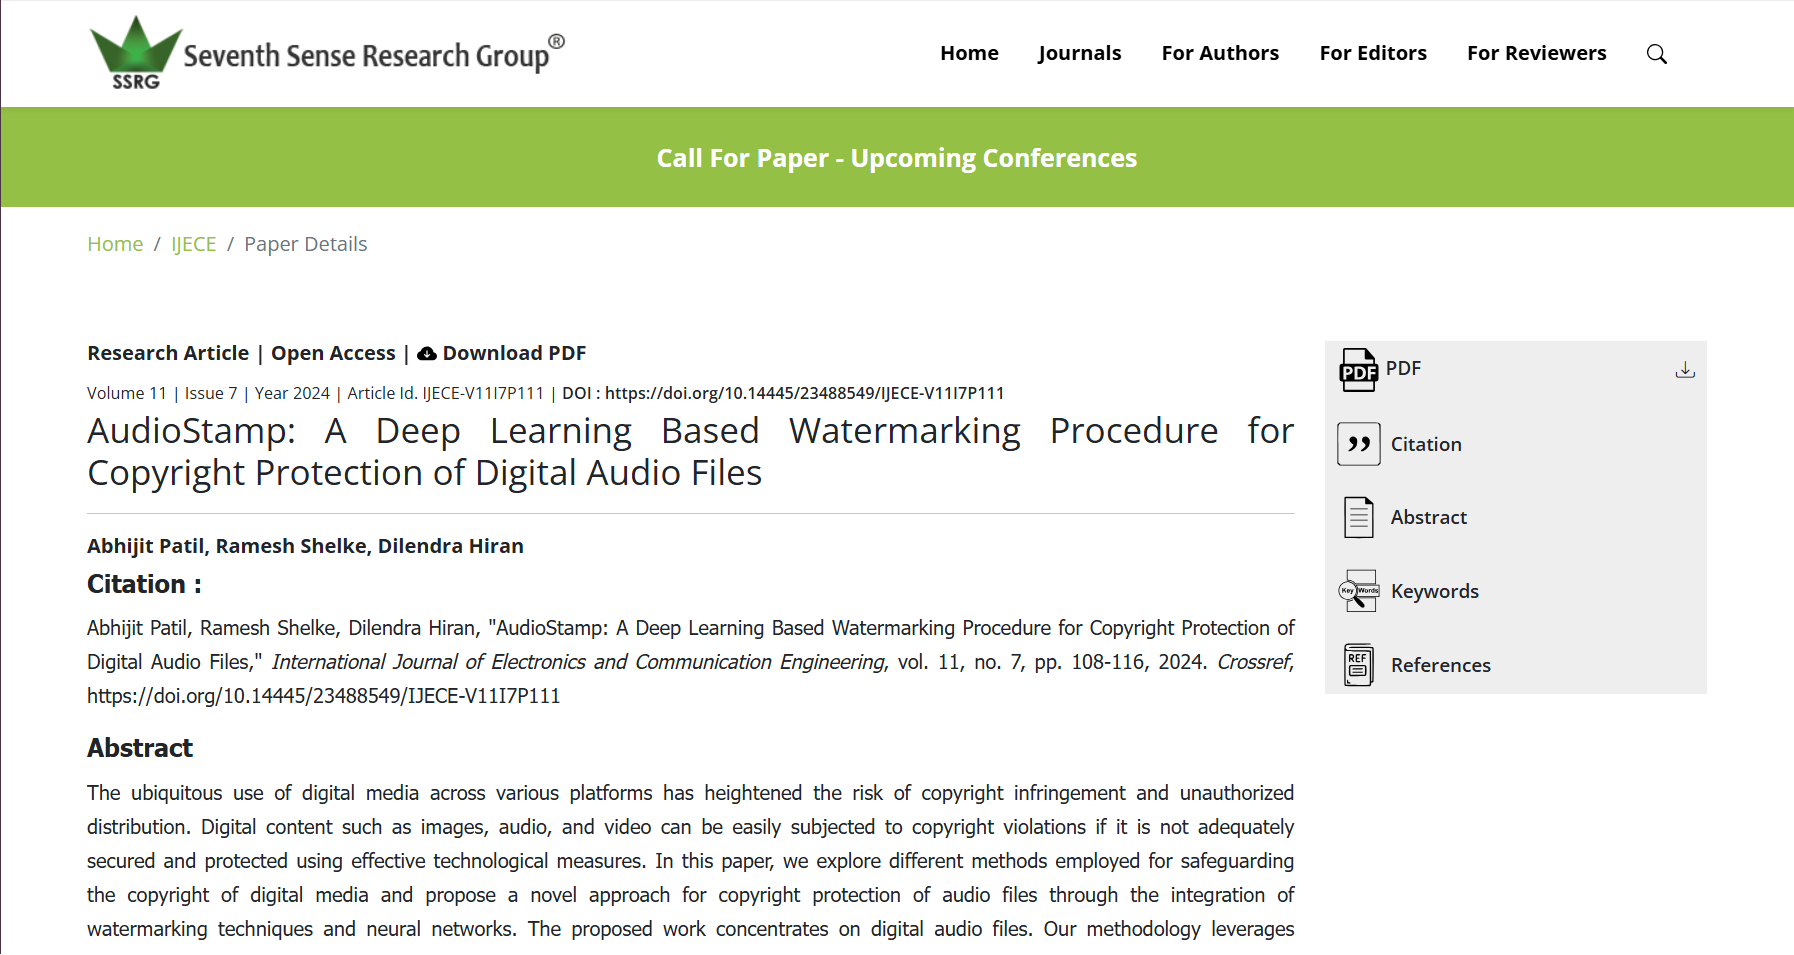
\includegraphics[width=0.9\textwidth]{captura2.png} \end{center}
\clearpage

% ARTÍCULO 3
\section*{3. Patil et al. (2023) - High-Confidence Computing}
\begin{center} 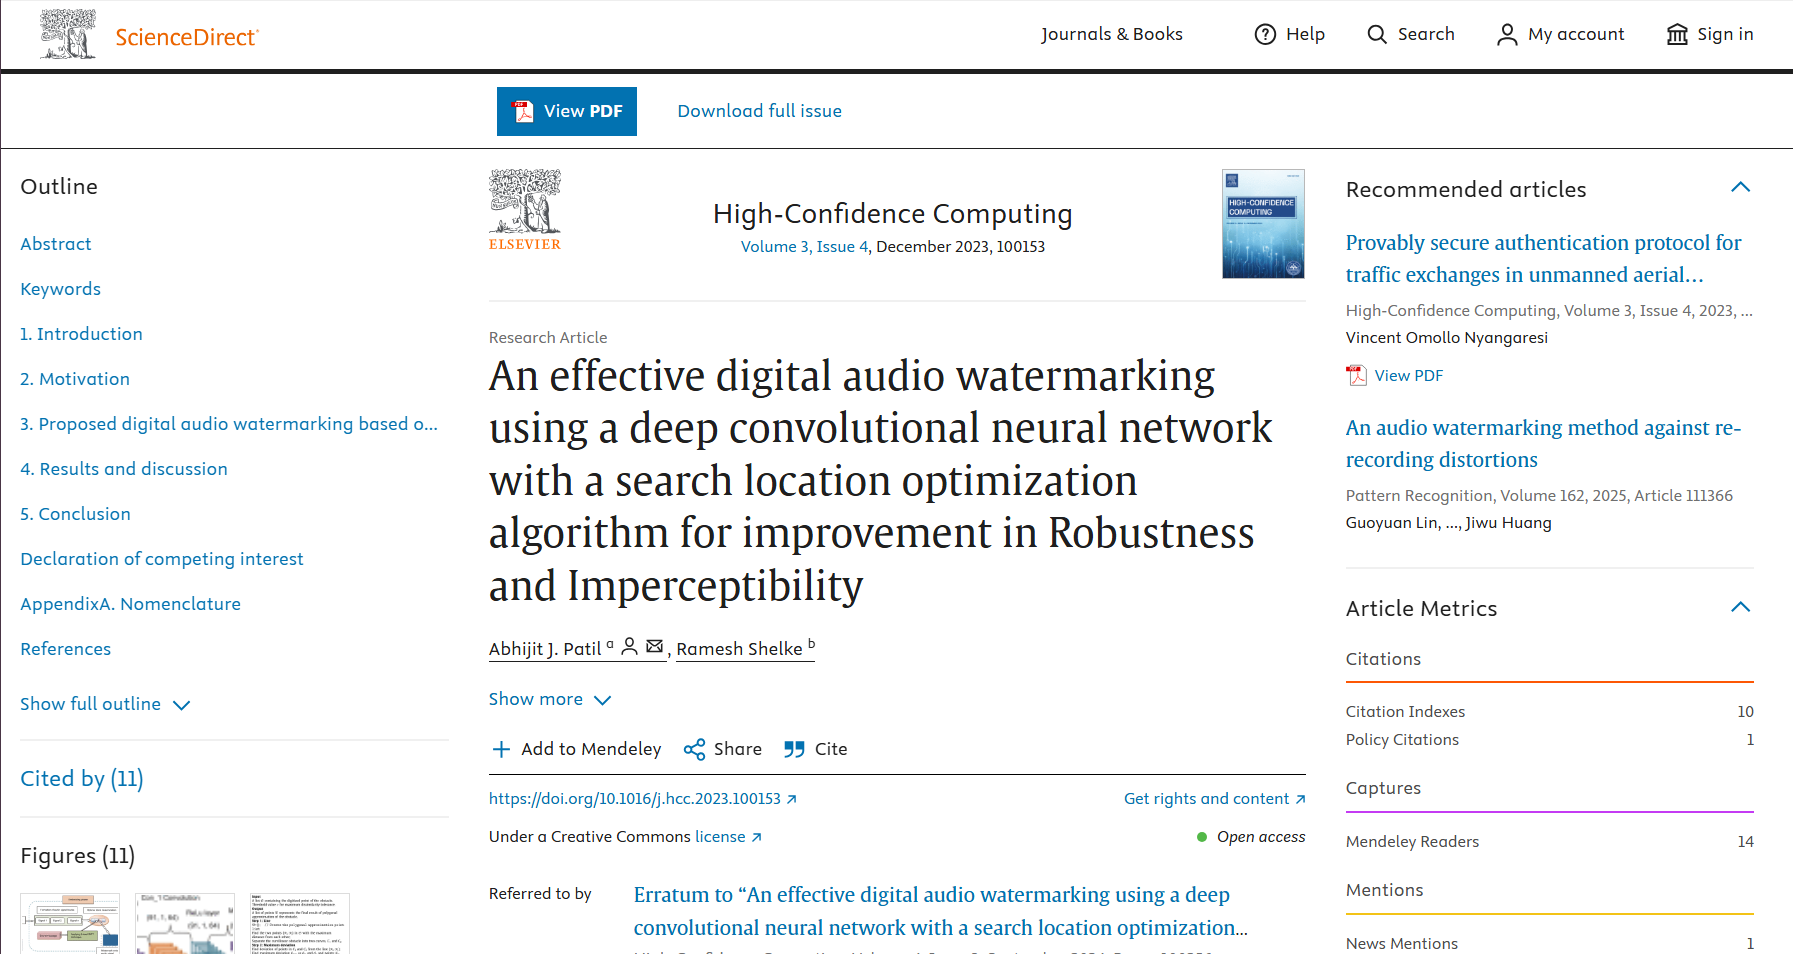
\includegraphics[width=0.9\textwidth]{captura3.png} \end{center}
\clearpage

% ARTÍCULO 4
\section*{4. Anon. (2025) - Academic Journal of Computing \& Information Science}
\begin{center} 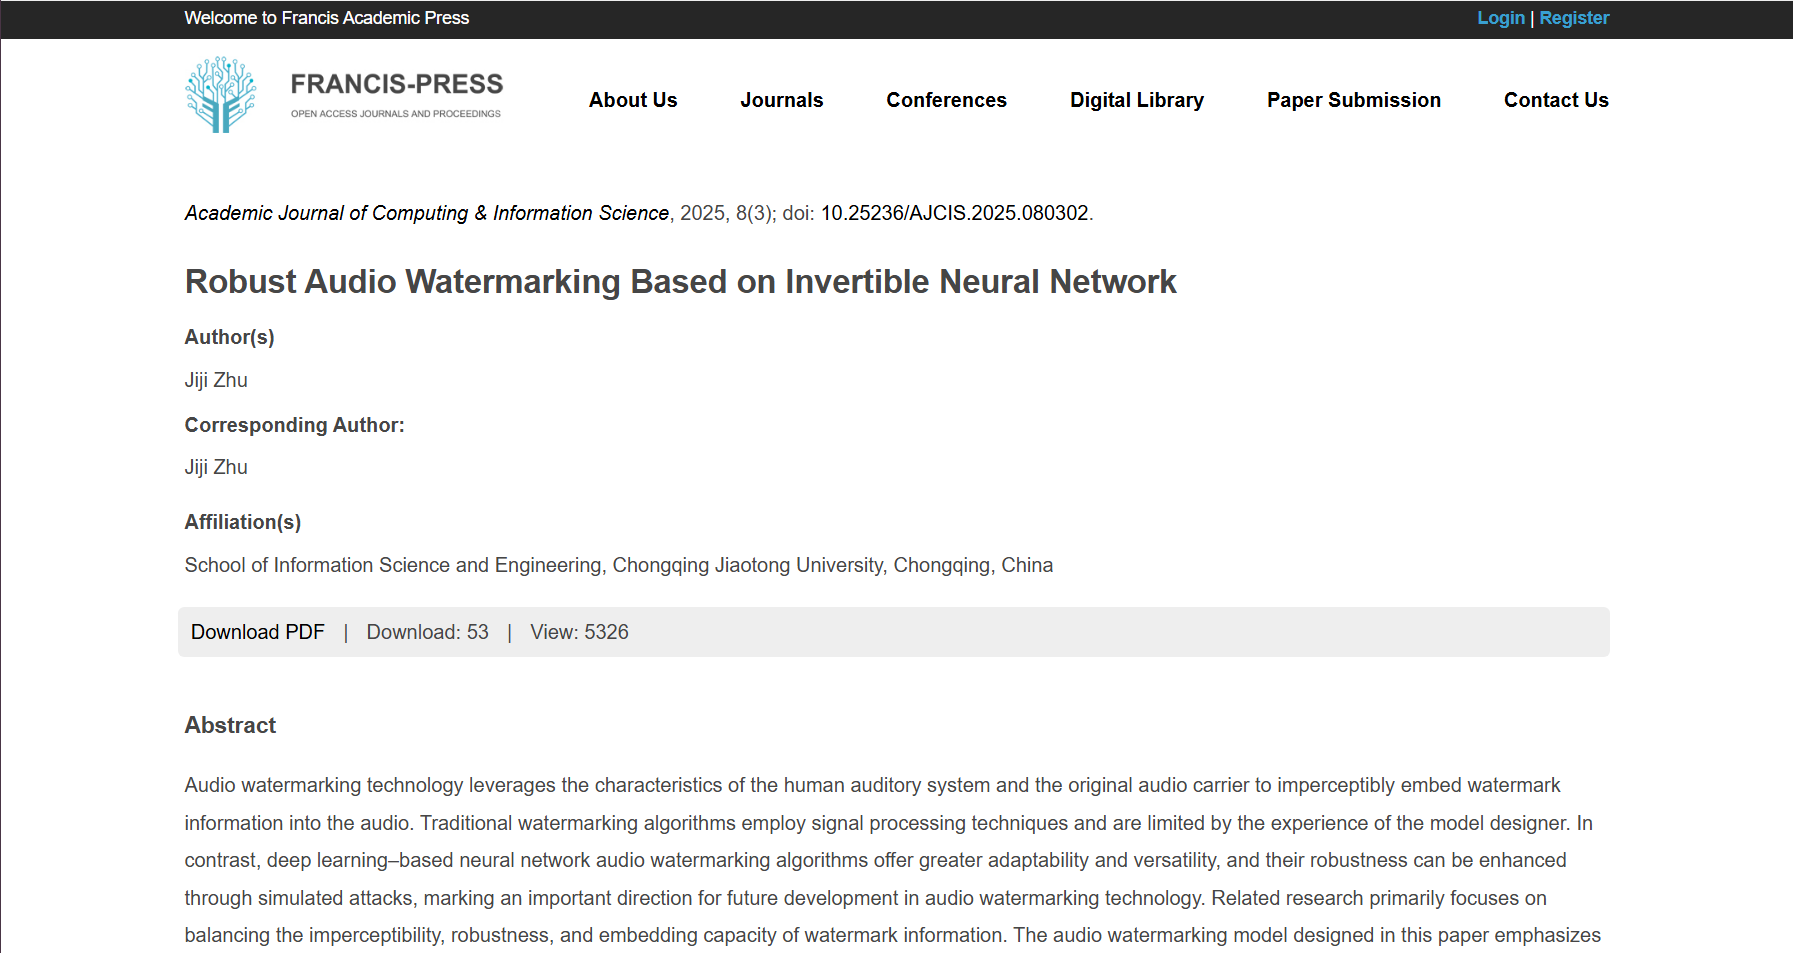
\includegraphics[width=0.9\textwidth]{captura4.png} \end{center}
\clearpage

% ARTÍCULO 5
\section*{5. Li et al. (2025) - IEEE/ACM TASLP}
\begin{center} 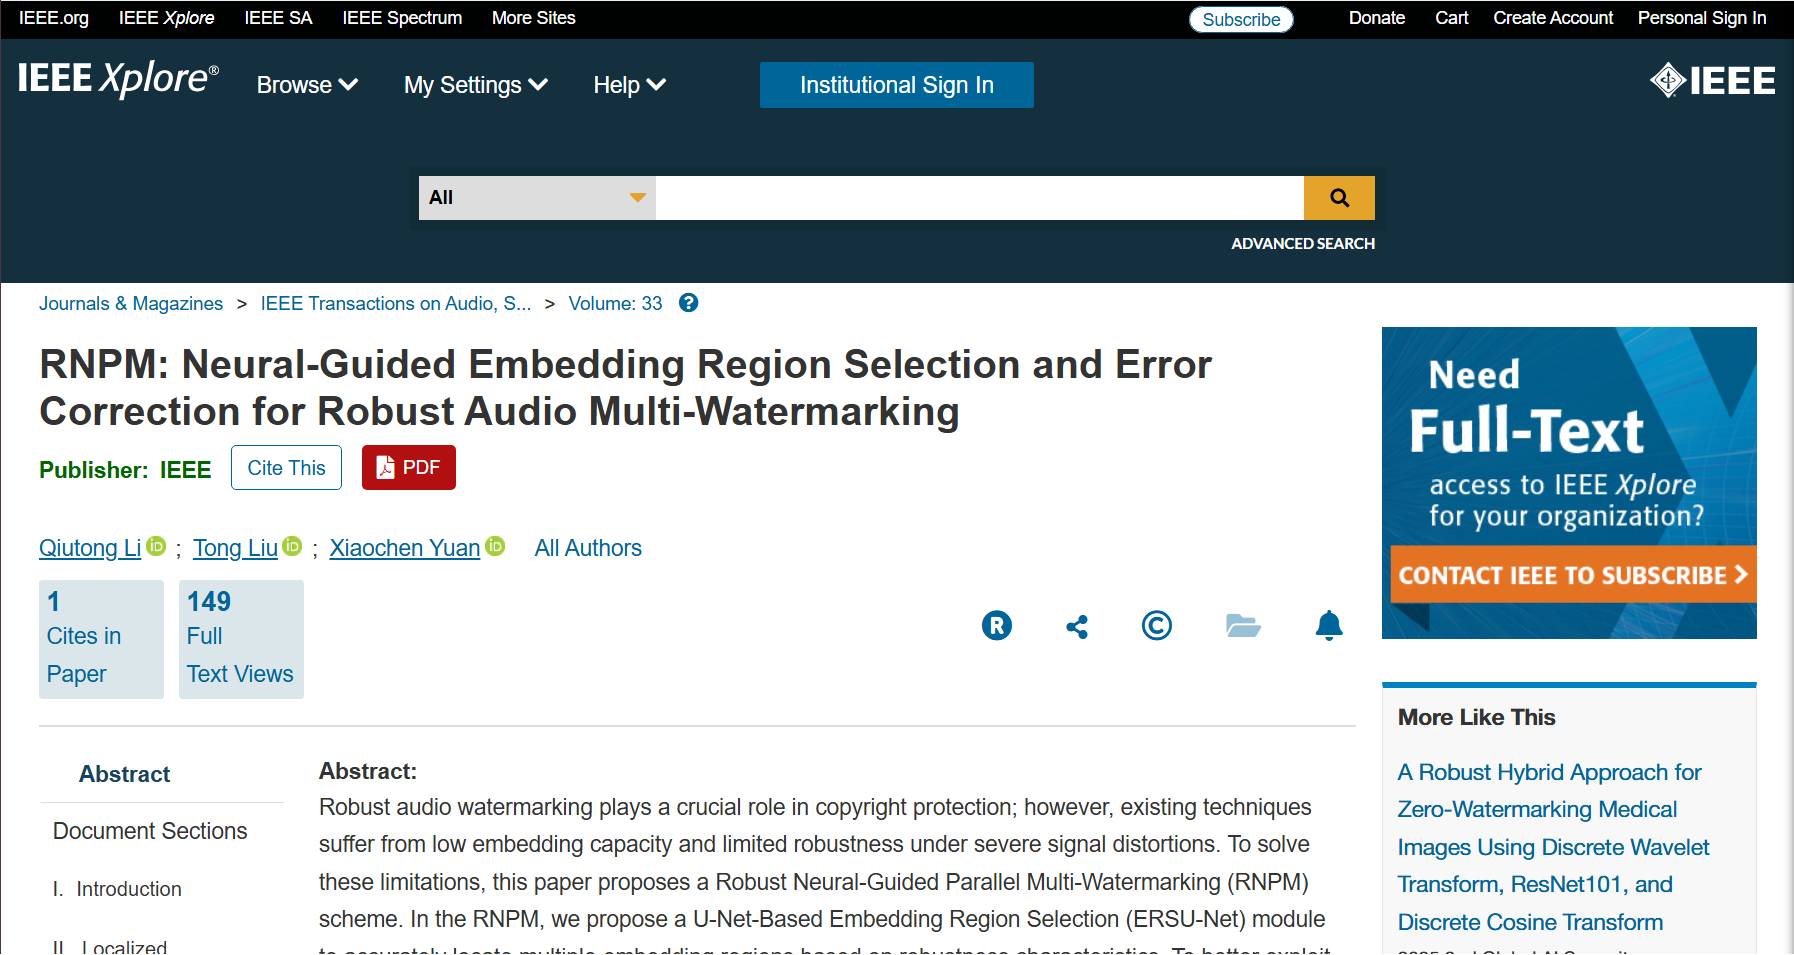
\includegraphics[width=0.9\textwidth]{captura5.png} \end{center}
\clearpage

% ARTÍCULO 6
\section*{6. Yang et al. (2014) - Int. J. of Computational Intelligence Systems}
\begin{center} 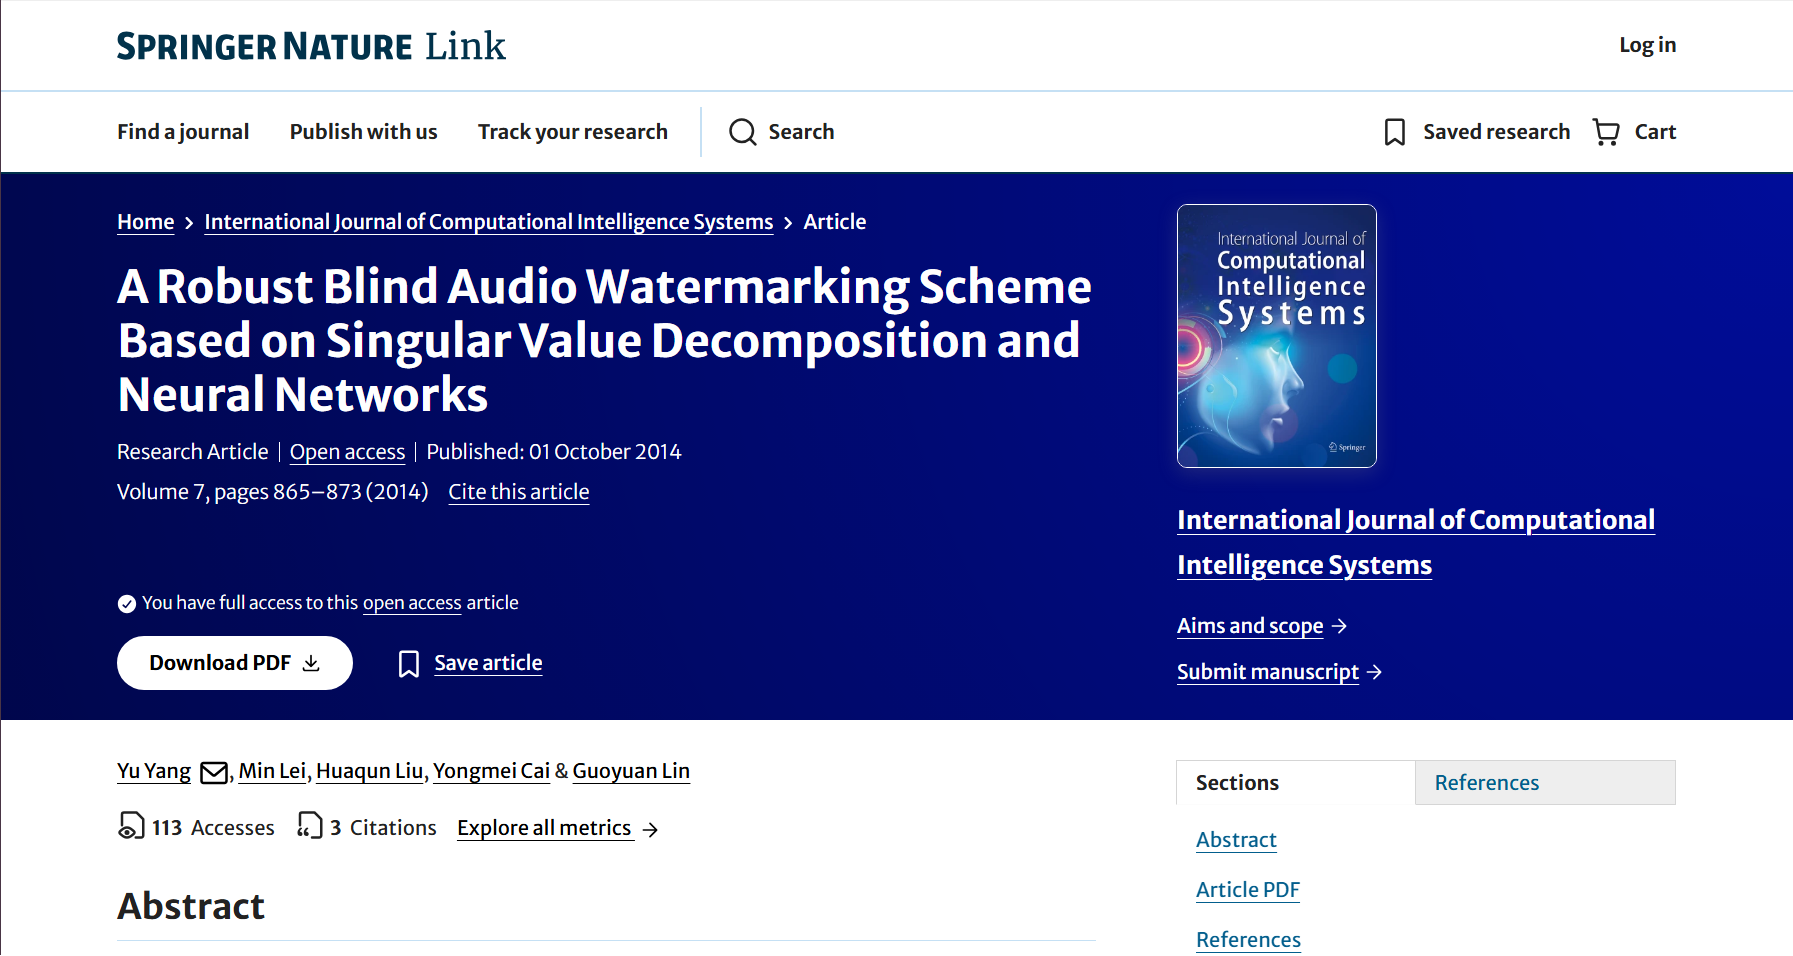
\includegraphics[width=0.9\textwidth]{captura6.png} \end{center}
\clearpage

% ARTÍCULO 7
\section*{7. Al-Haj (2014) - EURASIP Journal}
\begin{center} 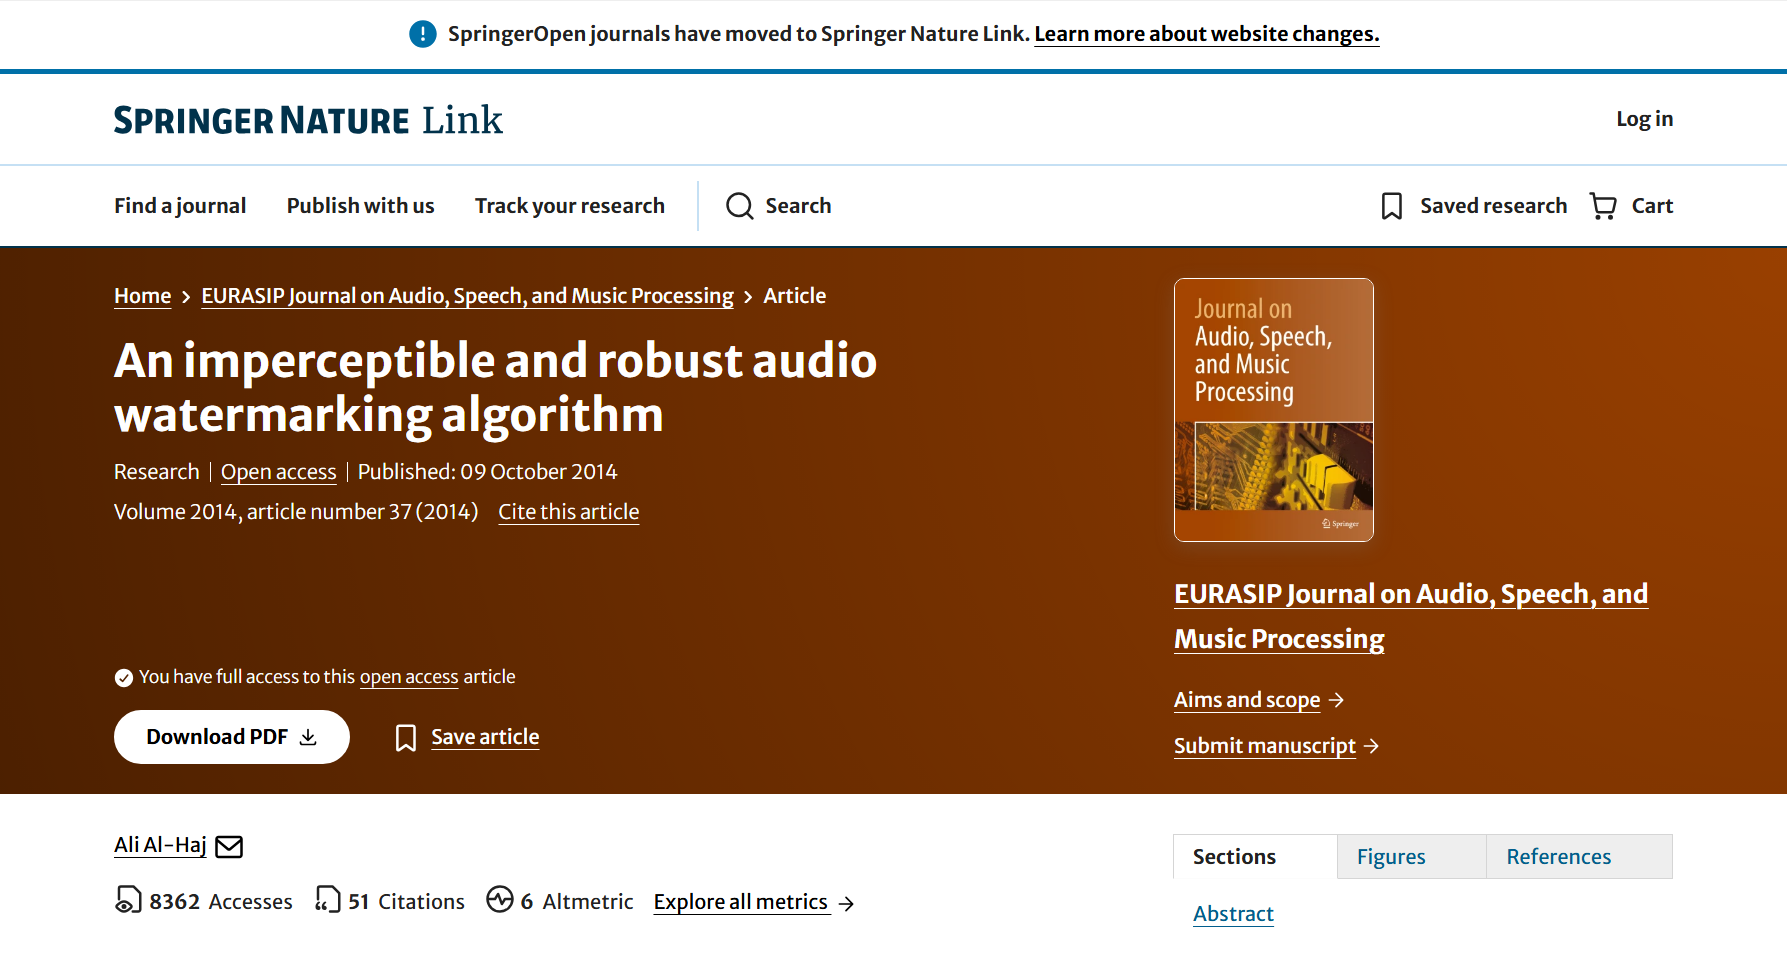
\includegraphics[width=0.9\textwidth]{captura7.png} \end{center}
\clearpage

% ARTÍCULO 8
\section*{8. Khaldi et al. (2013) - IEEE TASLP}
\begin{center} 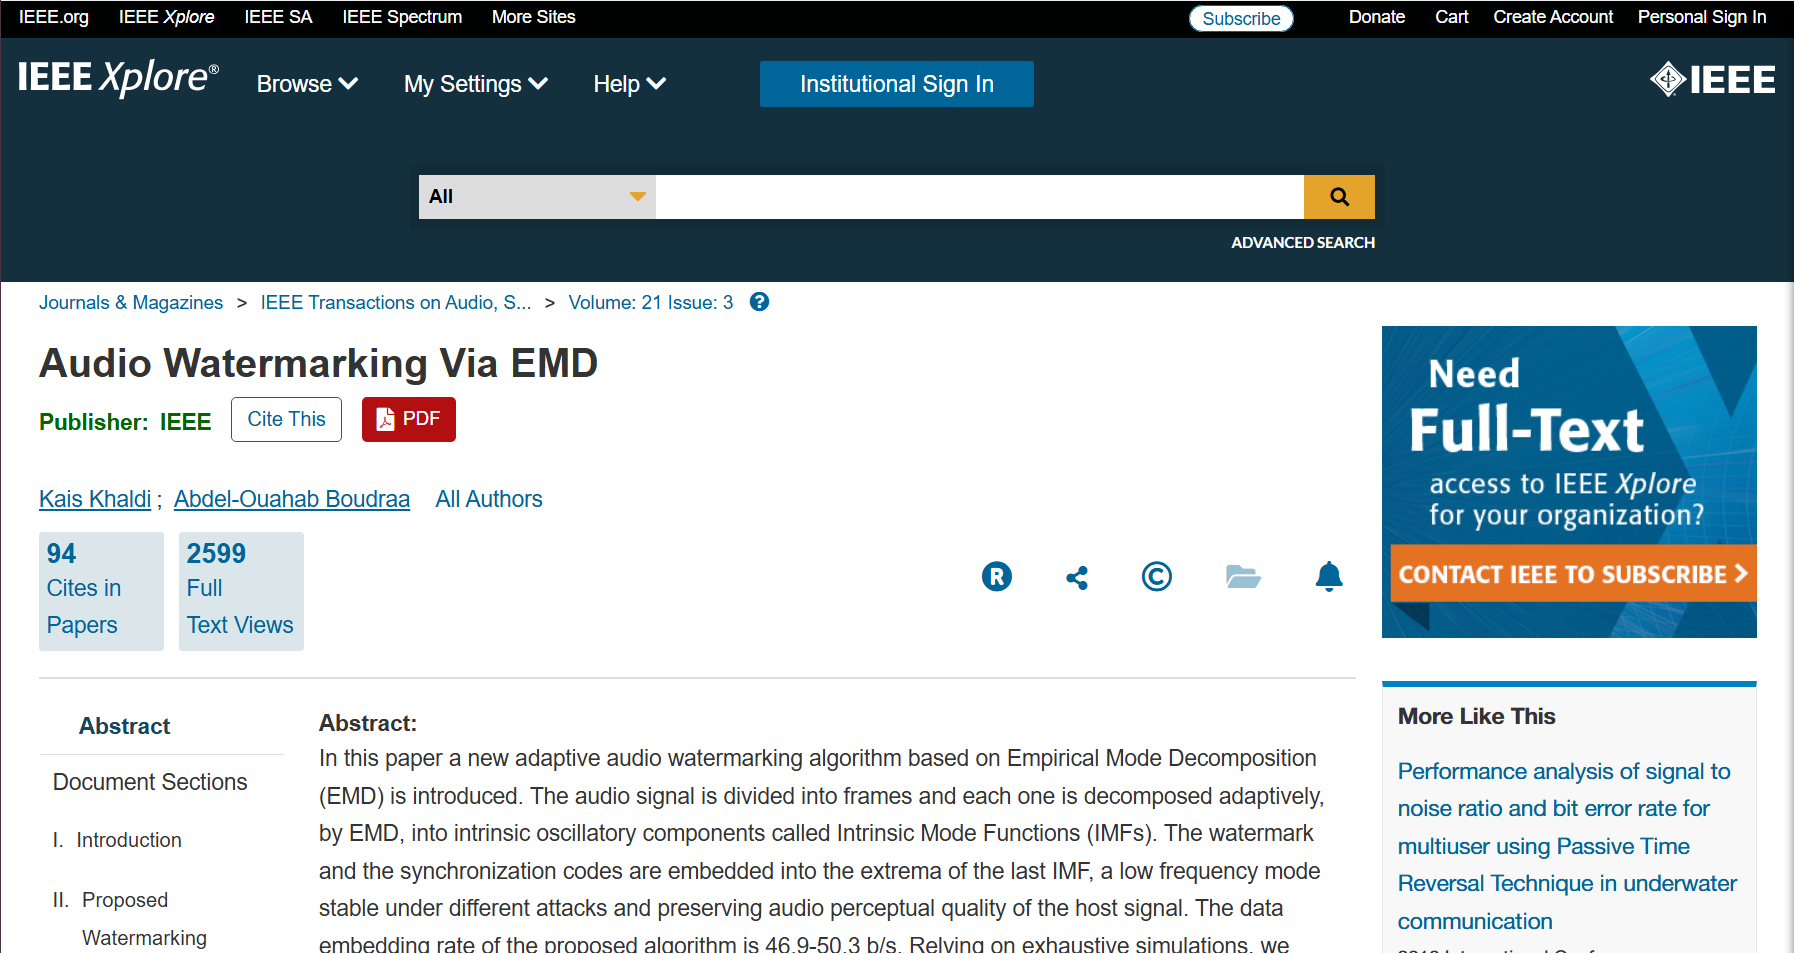
\includegraphics[width=0.9\textwidth]{captura8.png} \end{center}
\clearpage

% ARTÍCULO 9
\section*{9. Nishimura (2012) - IEEE TASLP}
\begin{center} 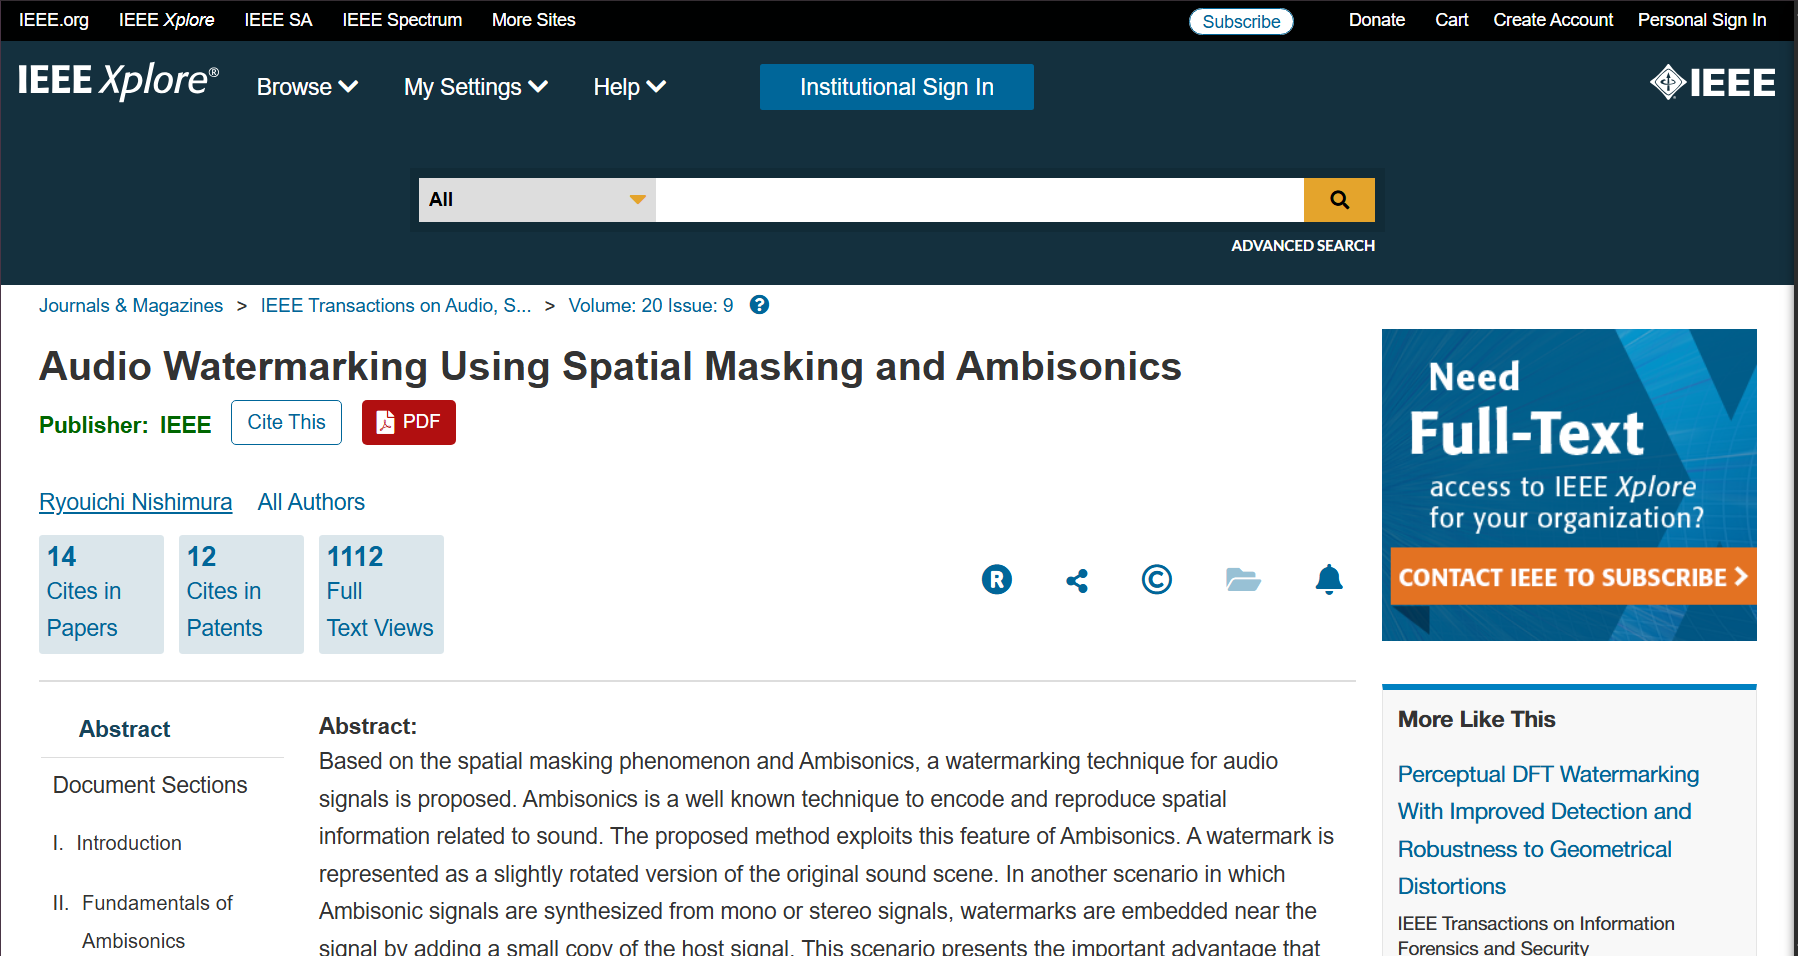
\includegraphics[width=0.9\textwidth]{captura9.png} \end{center}
\clearpage

% ARTÍCULO 10
\section*{10. Kanhe y Gnanasekaran (2018) - EURASIP Journal}
\begin{center} 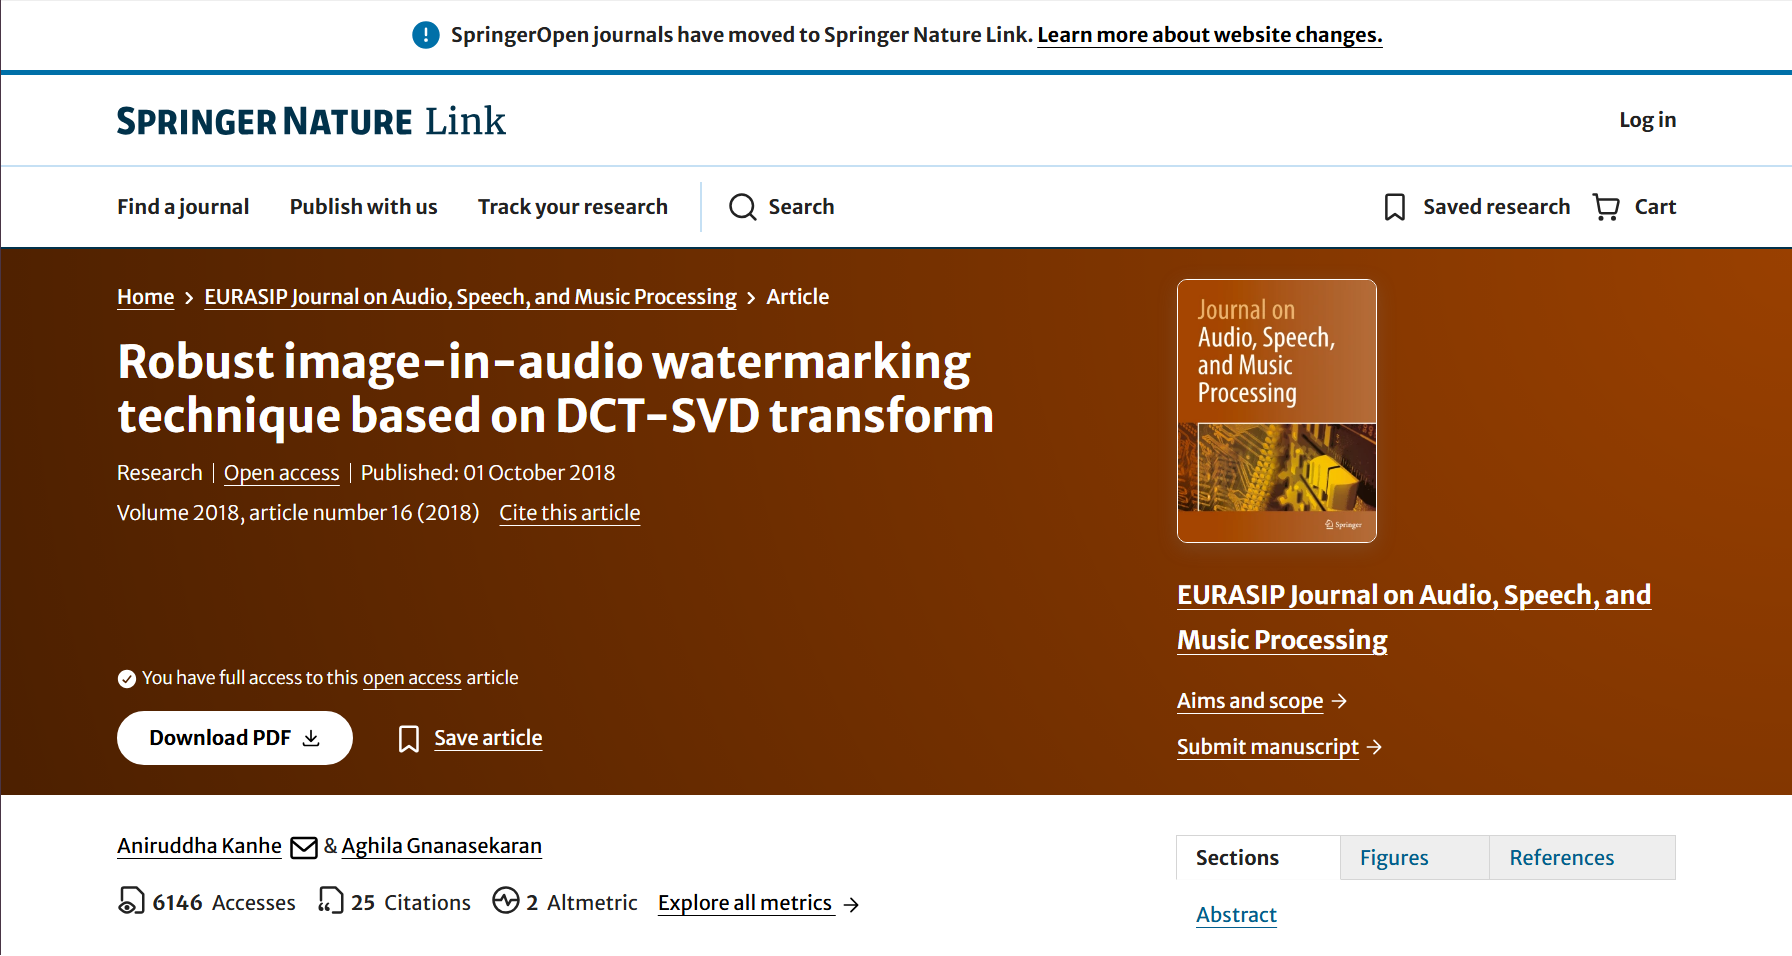
\includegraphics[width=0.9\textwidth]{captura10.png} \end{center}
\clearpage

\end{document}
